\chapter{\dspot: A Test Amplification Technique}
\label{chap:dspot}

\begin{chaptersummary}
		In this chapter, I expose the major output of this thesis: \dspot.
		\dspot is a test amplification tool that have the ambition to improve the test suite of real projects.
		\dspot achieves this by providing a set of automated procedures done in three majors step:
		\begin{enumerate}
			\item it modifies the test inputs in order to trigger new behavior.
			\item it generates assertions to verify the new behavior of the program.
			\item it selects amplified test methods according to a specific test-criterion such as branch coverage.
		\end{enumerate}
	
		\dspot's output is a set of amplified test methods that improve the original test suite according to the specified test-criterion.
		
		In this chapter, I first define key concepts in \autoref{sec:dspot:definitions};
		Then, I expose an overview of \dspot with its principle, input\& output, and its workflow in \autoref{sec:dspot:overview};
		Followed by the explanation of \dspot's algorithm in \autoref{sec:dspot:algorithm};
		Then, I detail the implementation and the ecosystem of \dspot in \autoref{sec:dspot:implemention}
		Eventually, I conclude this chapter in \autoref{sec:dspot:conclusion}
\end{chaptersummary}

\minitoc

\graphicspath{{.}{chapitres/dspot/}}

As mentioned in the previous chapter (see \autoref{chap:sota}), developers are mandated to build strong test suite in parallel of their application.
This reinforces the confidence that they have in the correctness of their application.

However, test suite are not the first objective and thus make it secondary.
Their development are focused on regular cases on the way that the program should behave.
In addition to this, developers may cut corners because of lack of time, expertise or discipline.

In the literature, one can find a lot of work trying to solve this issue, such as test suite generation or test suite evolution.
Test amplification is one of them.
However, the surveyed works present problems, in particular generalization of result, test amplification according to a multiple changes, scaling-up and assessment of the result by external real developers.

In this chapter, I expose the major output of this thesis: \dspot.
The ambitious with \dspot is to provide an open-source tool that would amplify the test suite.
Also, I developed \dspot in a way that it support real software, it can be used in the context of continuous integration.

\section{Definitions}
\label{sec:dspot:definitions}

I first define the core terminology of \dspot in the context of object-oriented Java programs.

\textbf{Test suite} is a set of test classes.

\textbf{Test class} is a class that contains test methods. 
A test class is neither deployed nor executed in production.

\textbf{Test method} or \textbf{test case} is a method that sets up the system under test into a specific state and checks that the actual state at the end of the method execution is the expected state.

\textbf{Unit test} is a test method that specifies a targeted behavior of a program. 
Unit tests are usually independent from each other and execute a small portion of the code, \ie a single unit or a single component of the whole system.

\textbf{System test} or \textbf{Integration test} is a test method that specifies a large and complex behavior of a program.
System tests are usually large and use a lot of different components of the program.

\textbf{Test-criterion} is a measure of the quality of the test suite according to an engineering goal.
For instance, one can measure the execution speed of its test suite, and consider that the faster it is executed the better it is.
The most popular is probably the execution coverage, which can be measured at different level: branches, statements, instructions.
It measures the proportion of the program that the test suite executes.
The larger is this proportion, the better is considered the test suite since it is likely to verify more behavior.

\textbf{Test inputs} are the first key component of test methods. 
The input setup part is responsible for driving the program into a specific state.
For instance, one creates objects and invokes methods on them to produce a specific state.

\textbf{Assertions} are the second key component of test methods. 
The assertion part is responsible for assessing that the actual behavior of the program corresponds to the expected behavior, the latter being called the oracle.
To do so, the assertion uses the state of the program, \ie all the observable values of the program, and compare it to expected values, usually hard-coded by developers.
If the actual observed values of the program state and the oracle are different (or if an exception is thrown), the test fails and the program is considered as incorrect.

\textbf{Amplified test suite} is an existing test suite to which amplified test methods has been added.

\textbf{Amplified test method} is a test method that has been amplified, \ie it has been obtained using an test amplification process and an existing test method.

\section{Overview}
\label{sec:dspot:overview}

\subsection{Principle}
\label{subsec:dspot:overview:principle}

\begin{figure}[h]
	\centering
	\fbox{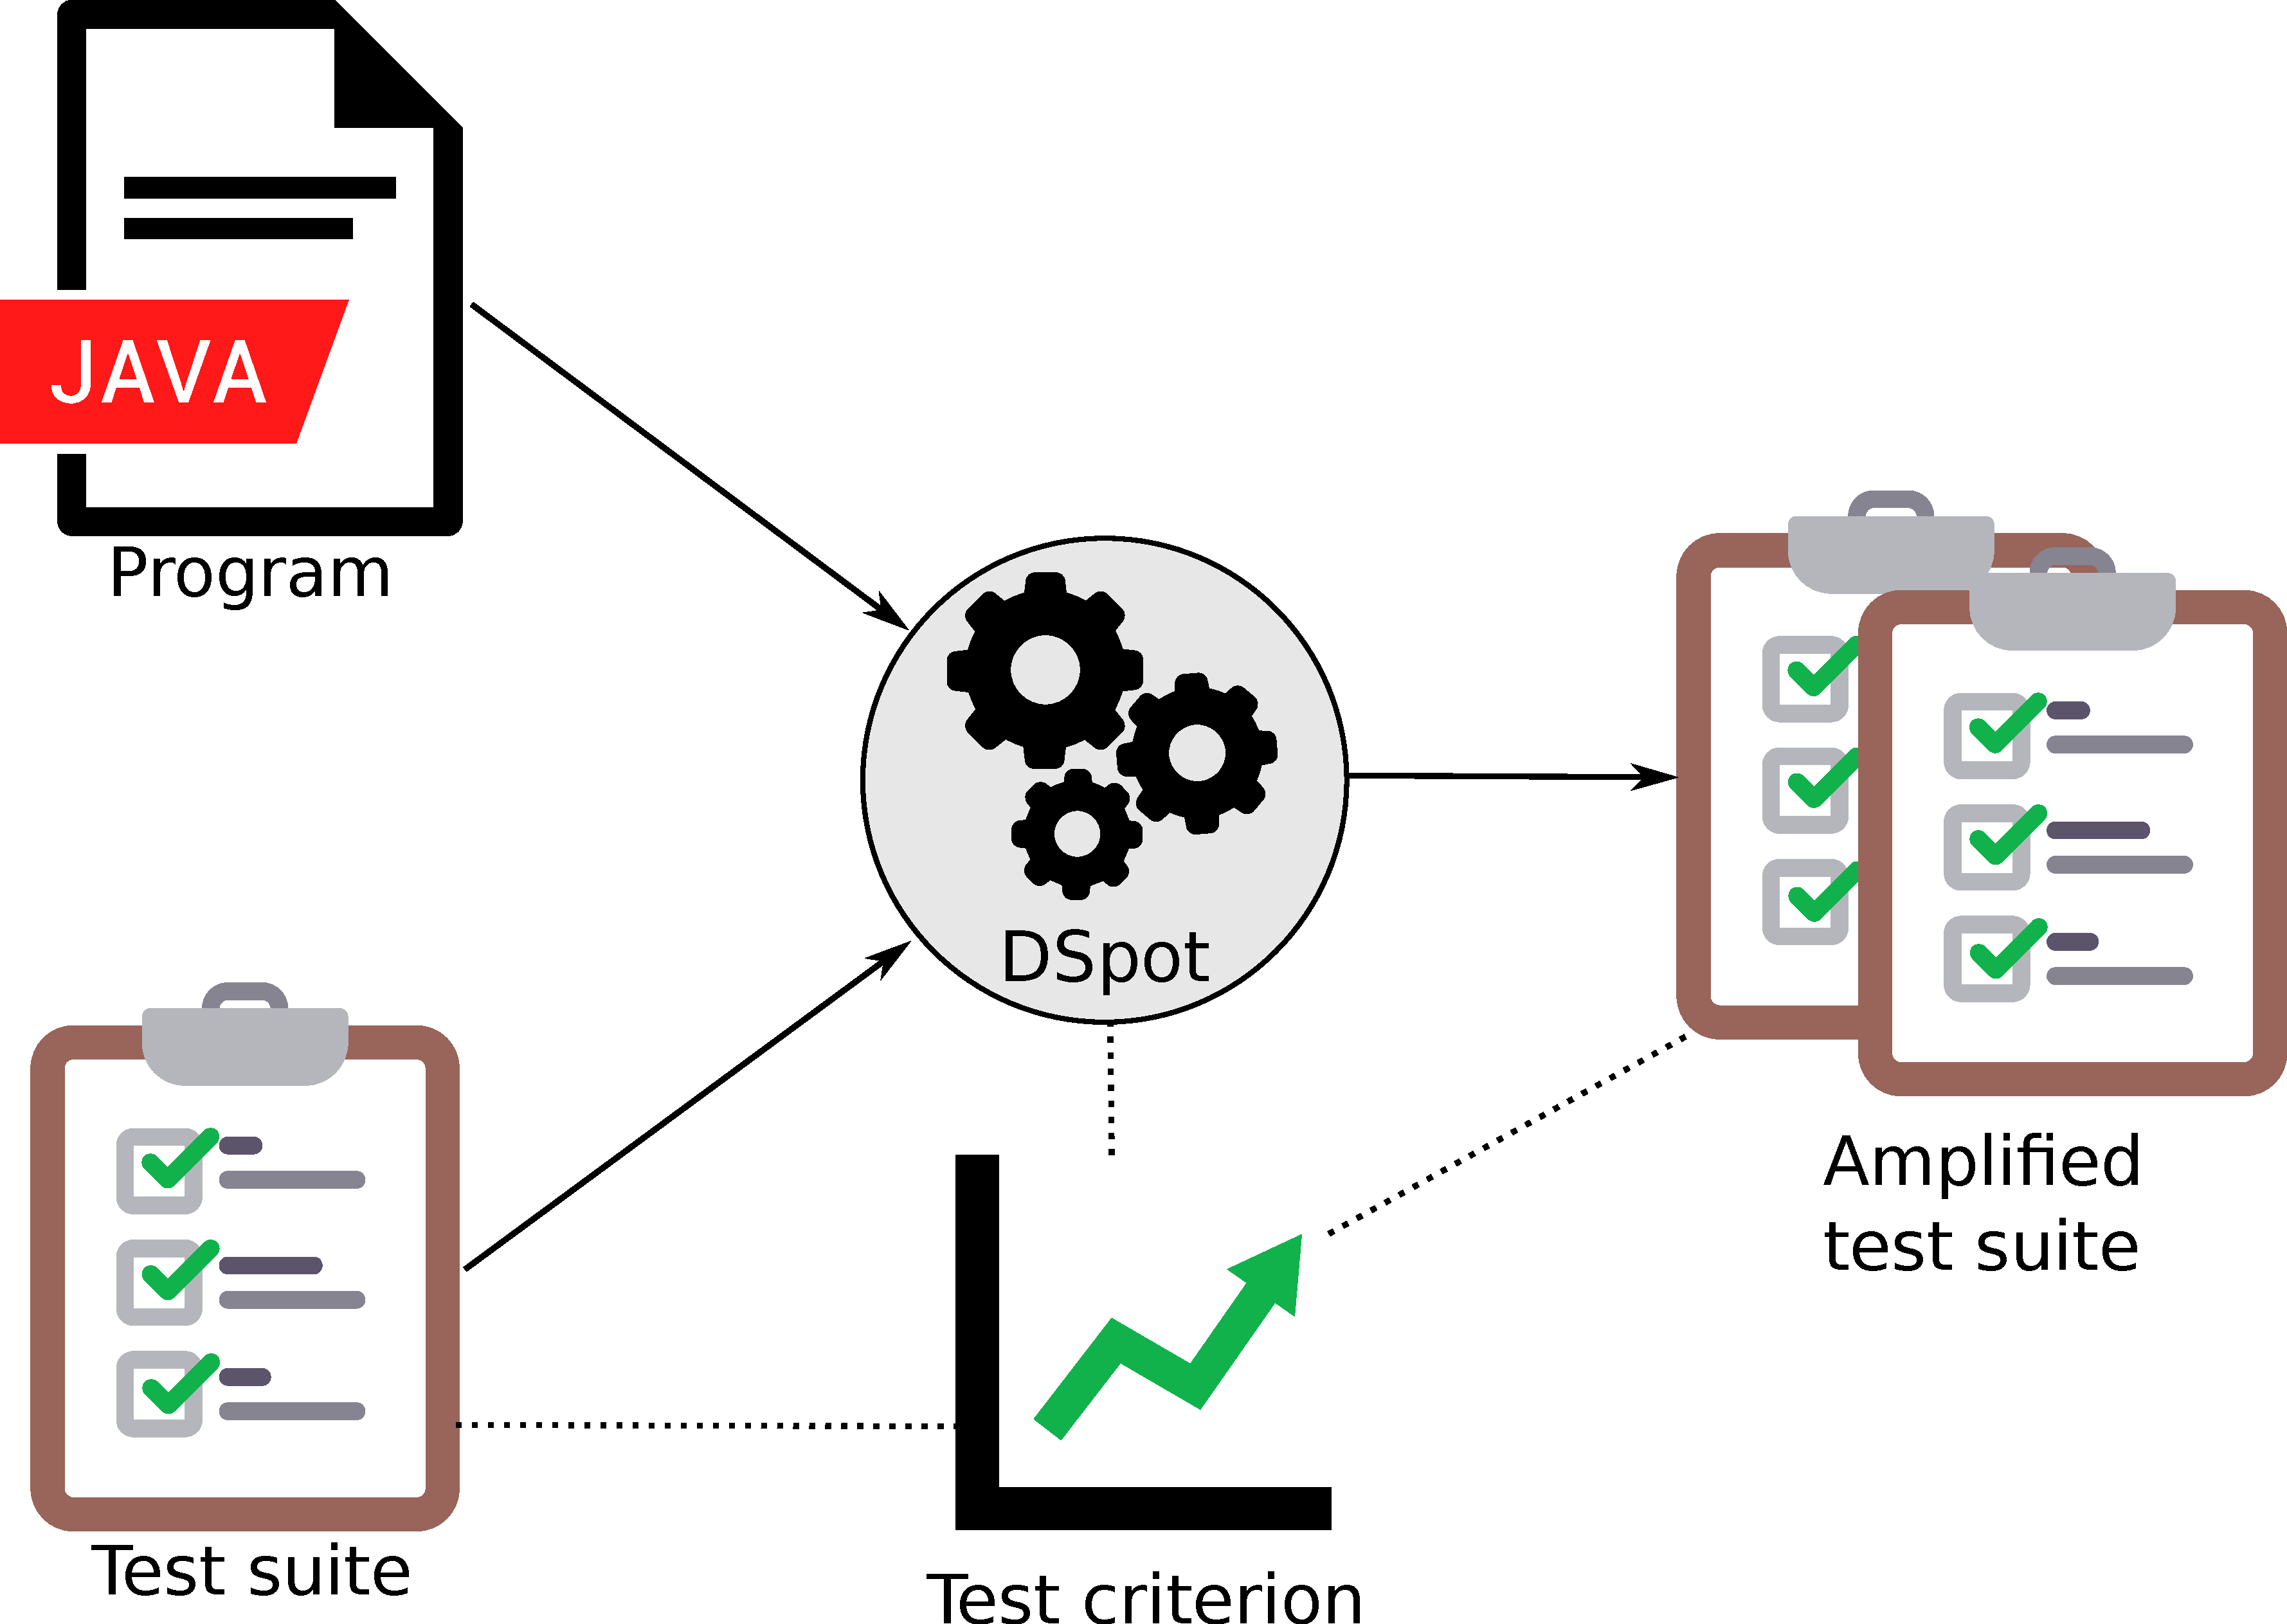
\includegraphics[width=.6\linewidth]{dspot_principle.pdf}}
	\caption{
		\dspot's principle: \dspot takes as input a program, an existing test suite, and a test-criterion. 
		\dspot outputs a set of amplified test methods.
		When added to the existing test suite, these amplified test methods increase the test-criterion, \ie the amplified test suite is better than the original one.
	}
	\label{fig:dspot:principle}
\end{figure}

DSpot is a test amplification tool.
Its goal is to improve an existing test suite according to a specific test-criterion.
DSpot takes as input the program, an existing test suite, and a test-criterion. 
The output of DSpot is a set of amplified test methods that are variants of existing test methods.
When added to the existing test suite, it create an amplified test suite.
This amplified test suite is better than the original test suite according to the test-criterion used during the amplification.
For instance, one amplifies its test suite using branch coverage as test-criterion.
This amplified test suite will execute more branches than the exiting test suite, \ie the one without amplified test methods.
In \dspot there are for now 3 test-criterion available:
1) keeping amplified test methods that increase the \ms;
2) keeping amplified test methods that increase the instruction coverage;
3) keeping amplified test methods that detect the behavioral difference between two versions of the same program.

\autoref{fig:dspot:principle} shows graphically the principle of \dspot.

\subsection{Input \& Output}
\label{subsec:dspot:overview:input-and-output}

\dspot's inputs are a program, a set of existing test methods and a test-criterion.
The program is used as ground truth: in \dspot we consider the program used during the amplification correct.
The existing test methods are used as a seed for the amplification.
\dspot applies transformation individually to these test methods in order to improve the overall quality of the test suite with respect to the specified test-criterion.

\dspot produces variants of the test methods provided as input.
These variants are called amplified test methods, since there are test methods that has been obtained using an amplification process.
These amplified test methods are meant to be added to the test suite.
By adding amplified test methods to the existing test suite, it creates an amplified test suite that improves the overall test suite quality.
By construction, the amplified test suite is better than the original one with respect to the specified criterion.

An amplified test method's integration can be done in two way:
1) the developer integrates as it is the amplified test method into the test suite;
2) the developer integrate only the changes between the original test method and the amplified test method.
This enrich directly an existing test method.

\begin{figure}[h]
	\centering\fbox{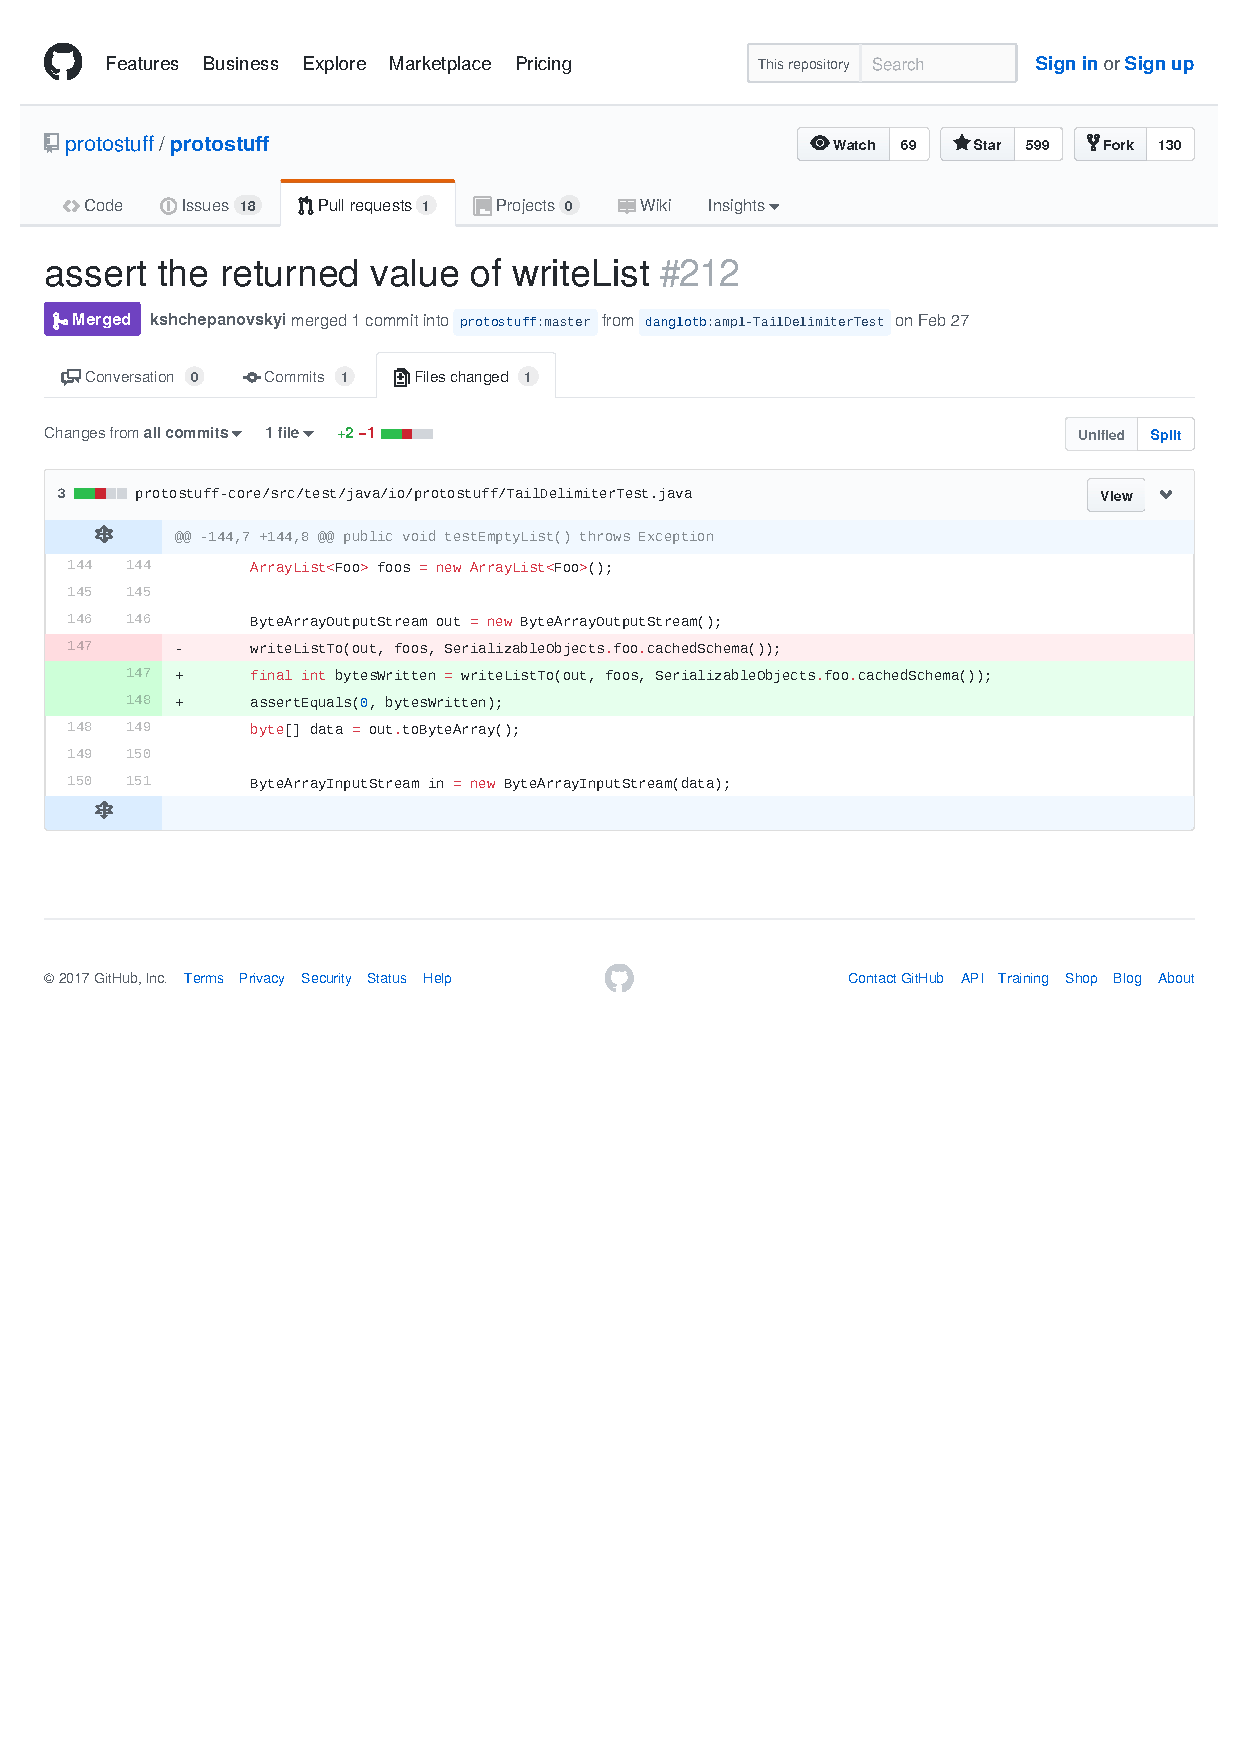
\includegraphics[width=0.98\textwidth, trim=4.15cm 17.52cm 4.05cm 10.76cm, clip]{protostuff.pdf}}
	\caption{Example of what \dspot produces: a diff to improve an existing test case.}
	\label{fig:diff-protostuff}
\end{figure}

\autoref{fig:diff-protostuff} shows an example of changes' set obtained using DSpot.

By construction, all \dspot's amplification can be represented as a diff on an existing test method since amplified test methods are variants of existing ones.

\subsection{Workflow}
\label{subsec:dspot:overview:workflow}

\begin{figure}[h]
	\centering\fbox{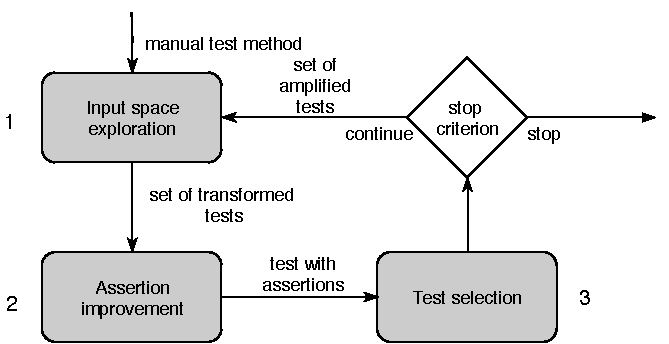
\includegraphics{dspot-workflow.pdf}}
	\caption{DSpot's workflow in three main steps: 
		1) the modification of test code's inputs, called ``input space exploration''; 
		2) the addition of new assertions called ``assertion improvement''; 
		3) the amplified test methods selection according to a test-criterion.
	}
	\label{fig:dspot-workflow}
\end{figure}

The main workflow of \dspot is composed of 3 main phases:
1) the modification of test code's inputs inspired by Tonella's technique~\cite{tonella}, called ``input space exploration''; 
this phase consists in modifying test values (\eg literals), objects and methods calls, the underlying details will be explained in \autoref{subsec:dspot:algorithm:input-space-exploration};
2) the addition of new assertions per Xie's technique~\cite{Xie2006}, this phase is called ``assertion improvement''
The behavior of the system under test is considered as the oracle of the assertion, see \autoref{subsec:dspot:algorithm:new-assertions}.
In \dspot, the combination of both techniques, \ie the combination of input space exploration and assertion improvement is called ``test amplification'';
3) the amplified test methods selection according to a given test-criterion, \eg branch coverage.
Eventually, \dspot either stops or continues to apply test amplification, according to a pre-defined stop-criterion.
By doing this, \dspot stacks the transformation of test methods.
In other words, \dspot amplifies already amplified test methods, which is possible because \dspot's output are real test methods.

In \dspot, the used stop-criterion is a number of iteration.
However, one can imagine others kinds of stop-criterion such as a time budget, a test-criterion goal(\eg reach 50\% of \ms) or a finite number of amplified test methods.

\subsection{Test method example}
\label{subsec:dspot:overview:appliance-to-unit-test}

\dspot amplifies Java program's test methods, which are typically composed of two parts: test inputs and assertions, see \autoref{sec:dspot:definitions}.

\autoref{lst:archetype} illustrates an archetypal example of such a test case: 
first, from line \autoref{input-begin} to line \autoref{input-end}, the test input is created through a sequence of object creations and method calls; 
then, at line \autoref{test}, the tested behavior is actually triggered; 
the last part of the test case at \autoref{assertion-1} and \autoref{assertion-2}, the assertion part, specifies and checks the conformance of the observed behavior with the expected one.
Note that this notion of call sequence and complex objects is different from test inputs consisting only of primitive values.

\begin{lstlisting}[caption={An example of an object-oriented test case  (inspired from Apache Commons Collections)},label=lst:archetype,float,language=java,numbers=left] 
testIterationOrder() {
// contract: the iteration order is the same as the insertion order

TreeList tl=new TreeList(); (*@\label{input-begin}@*)
tl.add(1);
tl.add(2); (*@\label{input-end}@*)

ListIterator it = tl.listIterator();(*@\label{test}@*)

// assertions
assertEquals(1, it.next().intValue());(*@\label{assertion-1}@*)
assertEquals(2, it.next().intValue());(*@\label{assertion-2}@*)
}
\end{lstlisting}

\subsubsection{Best target test}
\label{subsubsec:dspot:overview:appliance-to-unit-test:target-test}

By the algorithm's nature, unit tests (vs integration test) are the best target for \dspot.
The reasons are behind the very nature of unit tests:
First, they have a small scope, which allow \dspot to intensify its search while an integration test, that contains a lot of code, would make \dspot explore the neighborhood in different ways.
Second, that is a consequence of the first, the unit tests are fast to be executed against integration test.
Since \dspot needs to execute multiple times the tests under amplification, it means that \dspot would be executed faster when it amplifies unit tests than when it amplified integration tests.

\section{Algorithm}
\label{sec:dspot:algorithm}
% ---------------------------------------------------------------------------------------
% input space exploration: INPUT GOAL
% ---------------------------------------------------------------------------------------
\subsection{Input Space Exploration Algorithm}
\label{subsec:dspot:algorithm:input-space-exploration}

\dspot aims at exploring the input space so as to set the program in new, never explored states. To do so, \dspot applies code transformations to the original manually-written test methods. 

\textbf{\Iampl} for Input Amplification, is the process of automatically creating new test input points from existing test input points.

\dspot uses three kinds of \Iampl.

\emph{1) Amplification of literals}: the new input point is obtained by changing a literal used in the test (numeric, boolean, string).
These transformations are summarized in \autoref{table:test-transformations}.

\begin{table}
	\label{table:test-transformations}
	\caption{Literal test transformations in \dspot}
	\centering
	\begin{tabular}{cl}
		\toprule
		Types & Operators\\
		\midrule
		\multirow{5}{*}{Number}
		&\cellcolor{gray!25}add 1 to an integer\\
		&minus 1 to an integer\\
		&\cellcolor{gray!25}replace an integer by zero\\
		&replace an integer by the maximum value (Integer.MAX\_VALUE in Java)\\
		&\cellcolor{gray!25}replace an integer by the minimum value (\texttt{Integer.MIN\_VALUE} in Java).\\
		\midrule
		Boolean &  	
		\begin{tabular}{l}
			negate the value.
		\end{tabular}\\
		\midrule
		\multirow{6}{*}{String}
		&\cellcolor{gray!25}replace a string with another existing string.\\
		&replace a string with white space, or a system path separator, or a system\\
		&file separator.\\
		&\cellcolor{gray!25}add 1 random character to the string.\\
		&remove 1 random character from the string.\\
		&\cellcolor{gray!25}replace 1 random character in the string by another random character.\\
		&replace the string with a random string of the same size.\\
		&\cellcolor{gray!25}replace the string with the \texttt{null} value.\\
		\bottomrule
	\end{tabular}
\end{table}

\emph{2) Amplification of method calls}: \dspot manipulates method calls as follows:
\dspot duplicates an existing method call; removes a method call;
or adds a new invocation to an accessible method with an existing variable as target.

\emph{3) Test objects}:
if a new object is needed as a parameter while amplifying method calls, \dspot creates a new object of the required type using the default constructor if it exists.
In the same way, when a new method call needs primitive value parameters, \dspot generates a random value.

For example, if an \Iampl is applied on the example presented in \autoref{lst:archetype}, it may generate a new method call on \emph{tl}.
In \autoref{lst:iampl-example}, the added method call is ``removeAll''.
Since \dspot changes the state of the program, existing assertions may fail. 
That is why it removes also all existing assertions.

\begin{lstlisting}[caption={An example of an \Iampl{}: the amplification added a method call to \emph{removeAll()} on \emph{tl}.},label=lst:iampl-example,float,language=java,numbers=left] 
testIterationOrder() {
	TreeList tl=new TreeList(); (*@\label{input-begin-iampl}@*)
	tl.add(1);
	tl.add(2);
	tl.removeAll();(*@\label{input-end-iampl}@*) // method call added
	
	// removed assertions
}
\end{lstlisting}

At each iteration, \dspot applies all kinds of \Iampl, resulting in a set of input-amplified test methods. 
From one iteration to another, \dspot reuses the previously amplified tests, and further applies \Iampl.
By doing this, \dspot explore more the input space.
The more iteration \dspot does, the more it explores, the more it takes time to complete.

% ---------------------------------------------------------------------------------------
% Assertion improvement
% ---------------------------------------------------------------------------------------
\subsection{Assertion Improvement Algorithm}
\label{subsec:dspot:algorithm:new-assertions}

To improve existing tests, \dspot adds new assertions as follows.

\textbf{\Aampl:} for Assertion Amplification, is the process of automatically creating new assertions.

In \dspot, assertions are added on objects from the original test case, as follows: 
1) it instruments the test methods to collect the state of a program after execution (but before the assertions), \ie it creates observation points. 
The state is defined by all values returned by getter methods.
2) it runs the instrumented test to collect the values.
This execution result in a map per test method, that gives the values from all getters.
3) it generates new assertions in place of the observation points, using the collected values as oracle. 
In addition, when a new test input sets the program in a state that throws an exception, \dspot produces a test asserting that the program throws a specific exception.

For example, let consider \Aampl on the test method of the example above. 

First, in \autoref{lst:aampl-example-1} \dspot instruments the test method to collect values, by adding method calls to the objects involved in the test case.

\begin{lstlisting}[caption={In \Aampl{}, the second step is to instrument and run the test to collect runtime values.},label=lst:aampl-example-1,float,language=java,numbers=left] 
testIterationOrder() {
	TreeList tl=new TreeList(); (*@\label{input-begin-aampl}@*)
	tl.add(1);
	tl.add(2);aampl
	tl.removeAll();(*@\label{input-end-aampl}@*)
	
	// logging current behavior
	Observations.observe(tl.size()); 
	Observations.observe(tl.isEmpty()); 
}
\end{lstlisting}

Second, the test with the added observation points is executed, and subsequently, \dspot generates new assertions based on the collected values. 
In \autoref{lst:aampl-example-2}, \dspot has generated two new assertions.

\begin{lstlisting}[caption={In \Aampl{}, the last step is to generate the assertions based on the collected values.},label=lst:aampl-example-2,float,language=java,numbers=left] 
testIterationOrder() {
	TreeList tl=new TreeList(); (*@\label{input-begin-aampl2}@*)
	tl.add(1);
	tl.add(2);
	tl.removeAll();(*@\label{input-end-aampl2}@*)
	
	// generated assertions
	assertEquals(0, tl.size()); // generated assertions
	assertTrue(tl.isEmpty()); // generated assertions
}
\end{lstlisting}

% ---------------------------------------------------------------------------------------
% algorithm
% ---------------------------------------------------------------------------------------
\subsection{Pseudo-algorithm}
\label{subsec:dspot:algorithm:pseudo-algo}

\begin{algorithm}[t]
	\begin{algorithmic}[1]
		\Require{Program $P$}
		\Require{Test suite $TS$}
		\Require{Test criterion $TC$}
		\Require{Input-amplifiers $amps$ to generate new test data input}
		\Require{$n$ number of iterations of \dspot's main loop}
		\Ensure{An amplified test suite $ATS$}
		\State{$ATS \leftarrow \emptyset$}
		\For{$t$ in $TS$}
		\State{$U \leftarrow generateAssertions\left(t\right)$}
		\State{$ATS \leftarrow \{ x \in U | \mbox{x improves TC} \}$}
		\State{$TMP \leftarrow ATS$}
		\For{$i = 0$ to $n$}
		\State{$V \leftarrow [ ]$}
		\For{$amp$ in $amps$}
		\State{$V \leftarrow V \cup amp.apply\left(TMP\right)$}
		\EndFor
		\State{$V \leftarrow generateAssertions\left(V\right)$}
		\State{$ATS \leftarrow ATS \cup \{ x \in V | \mbox{x improves TC} \}$}
		\State{$TMP \leftarrow V$}
		\EndFor
		\EndFor
		\Return{$ATS$}
	\end{algorithmic}
	\caption{Main amplification loop of \dspot.}
	\label{algo:dspot_main}
\end{algorithm}

\autoref{algo:dspot_main} shows the main loop of \dspot. 
\dspot takes as input a program $P$, its test suite $TS$ and a test-criterion $TC$. 
\dspot also uses an integer $n$ that defines the number of iterations and a set of input-amplifiers $amp$.
\dspot produces an amplified test suite $ATS$, \ie a better version of the input test suite $TS$ according to the specified test criterion $TC$.
First, \dspot initializes an empty set of amplified test methods $ATS$ that will be outputted (Line 1).
For each test case $t$ in the test suite $TS$ (Line 2), 
\dspot first tries to add assertions without generating any new test input (Line 3), method $generateAssertions\left(t\right)$ is explained in \autoref{subsec:dspot:algorithm:new-assertions}.
It adds to $ATS$ the tests that improve the test-criterion(Line 4).

Note that adding missing assertions is the elementary way to improve existing tests.
Consequently, in \dspot there are two modes, depending on the configuration:

1) \dspot executes only assertion amplification, if $n = 0$ or $amp = \emptyset $:

2) \dspot executes both input space exploration and assertion amplification, if $n > 0$ and $amp \ne \emptyset$

In the former mode, there is no exploration of the input space, resulting in a quick execution but less potential to improve the test-criterion.
In the latter mode, the exploration, depending on $n$, takes times but have more potential to improve the test-criterion.

\dspot initializes a temporary list of tests $TMP$ with elements from $ATS$, if any (Line 5).
Then it applies $n$ times the following steps (Line 6):
1) it applies each amplifier $amp$ on each tests of $TMP$ to build $V$ (Line 8-9 see \autoref{subsec:dspot:algorithm:input-space-exploration} \ie \Iampl);
2) it generates assertions on generated tests in $V$ (Line 11 see \autoref{subsec:dspot:algorithm:new-assertions}, \ie \Aampl);
3) it keeps the tests that improve the test-criterion(Line 12).
4) it assigns $V$ to $TMP$ for the next iteration. This is done because even if some amplified test methods in $V$ have not been selected, it can contain amplified test methods that will eventually be better in subsequent iterations.

\subsection{Flaky tests elimination}
\label{subsec:dspot:algorithm:flaky-test-elimination}
The input space exploration (see \autoref{subsec:dspot:algorithm:input-space-exploration}) may produce test inputs that results in non-deterministic executions.
This means that, between two independent executions, the state of the program is not the same.
Since \dspot generates assertions where the expected value is a hard coded value from a specific run (see \autoref{subsec:dspot:algorithm:new-assertions}), the generated test case may become flaky: it passes or fails depending on the execution and whether the expected value is obtained or not.

To avoid such flaky tests, \dspot run $f$ times each new test case resulting from amplification ($f$ = 3 in the default configuration). 
If a test fails at least once, \dspot throws it away. 
This procedure does not guarantee the absence of flakiness.
However, it gives incremental confidence: if the user wants more confidence, she can tell \dspot to run the amplified tests more times.

\section{Implementation}
\label{sec:dspot:implemention}

\dspot is implemented in Java.
It consists of 19295+ logical lines of code (as measured by cloc).
\dspot uses Spoon\cite{pawlak:hal-01169705} to analyze and transform the tests of the software application under amplification.

\subsection{Ecosystem}
\label{subsec:dspot:implemention:ecosystem}

For the sake of open-science, \dspot is made publicly available on Github\footnote{\url{https://github.com/STAMP-project/dspot}}.
This repository is animated by the community around \dspot.
It uses a pull-request based development to promote open-source contributions.

Since \dspot has been developed with the ultimate goal to serve developers in their task of testing their programs, I participated to the development of a rich ecosystem.

First, \dspot-maven is a maven plugin that allows developers to execute \dspot on their maven project without downloading anything.
This plugin allows also developers to configure \dspot inside their own pom with specific setup in order to automate the application of \dspot.

Second, STAMP's partners developed an Eclipse plugin and Jenkins plugin. 
The former allows developers to run \dspot inside Eclipse, with a friendly UI to configure it. 
The latter allows developers to run \dspot as a Jenkins jobs in order to integrate \dspot in their continuous integration service.

\section{Conclusion}
\label{sec:dspot:conclusion}

This chapter presents technical details about \dspot.
\dspot is a test amplification tool that improve the test suite.
\dspot works in three main steps:
\begin{enumerate}
	\item it modifies the test inputs in order to trigger new behavior.
	\item it generates assertions to verify the new behavior of the program.
	\item it selects amplified test methods according to a specific test-criterion such as branch coverage.
\end{enumerate}

\dspot's output is a set of amplified test methods that improve the original test suite according to the specified test-criterion.\\

In the two following chapters, I evaluate the performance of \dspot to improve existing test suite in two scenarios:

A first scenario where \dspot improve existing test suite of open-source projects from \gh.
\dspot's output is evaluated by external developers and the test-criterion to improve is the mutation score.

A second scenario where \dspot is enhanced to be executed inside the continuous in order to detect a behavioral changes introduced by commits done by developers on a version control platform such as \gh.